\section{Avaliação}

Uma avaliação preliminar da interface de usuário, utilizando o protótipo de média fidelidade foi realizada com um conjunto de cerca de cinco usuários, entre 20 e 30 anos, todos demonstraram satisfação para com o sistema e curiosidade pela implementação final.

O teste com um usuário de 52 anos foi realizado na versão final, o feedback apontou a boa praticidade no sistema, objetividade na apresentação de resultados e simplicidade na interface.

Outros testes de funcionamento do sistema foram realizados, a respeito do tratamento de erros internos ao servidor e lidando com páginas não encontradas pelo sistema, sempre apresentando uma página amigável ao usuário.

Algumas capturas da interface final são apresentadas na figura \ref{fig:desktop:final}, apresentando uma pergunta do banco de dados em \ref{fig:desktop:disease_real} e resultados em \ref{fig:desktop:results_real}.

\begin{figure}[htbp]
	\centering
	\begin{subfigure}{0.49\linewidth}
		\centering
		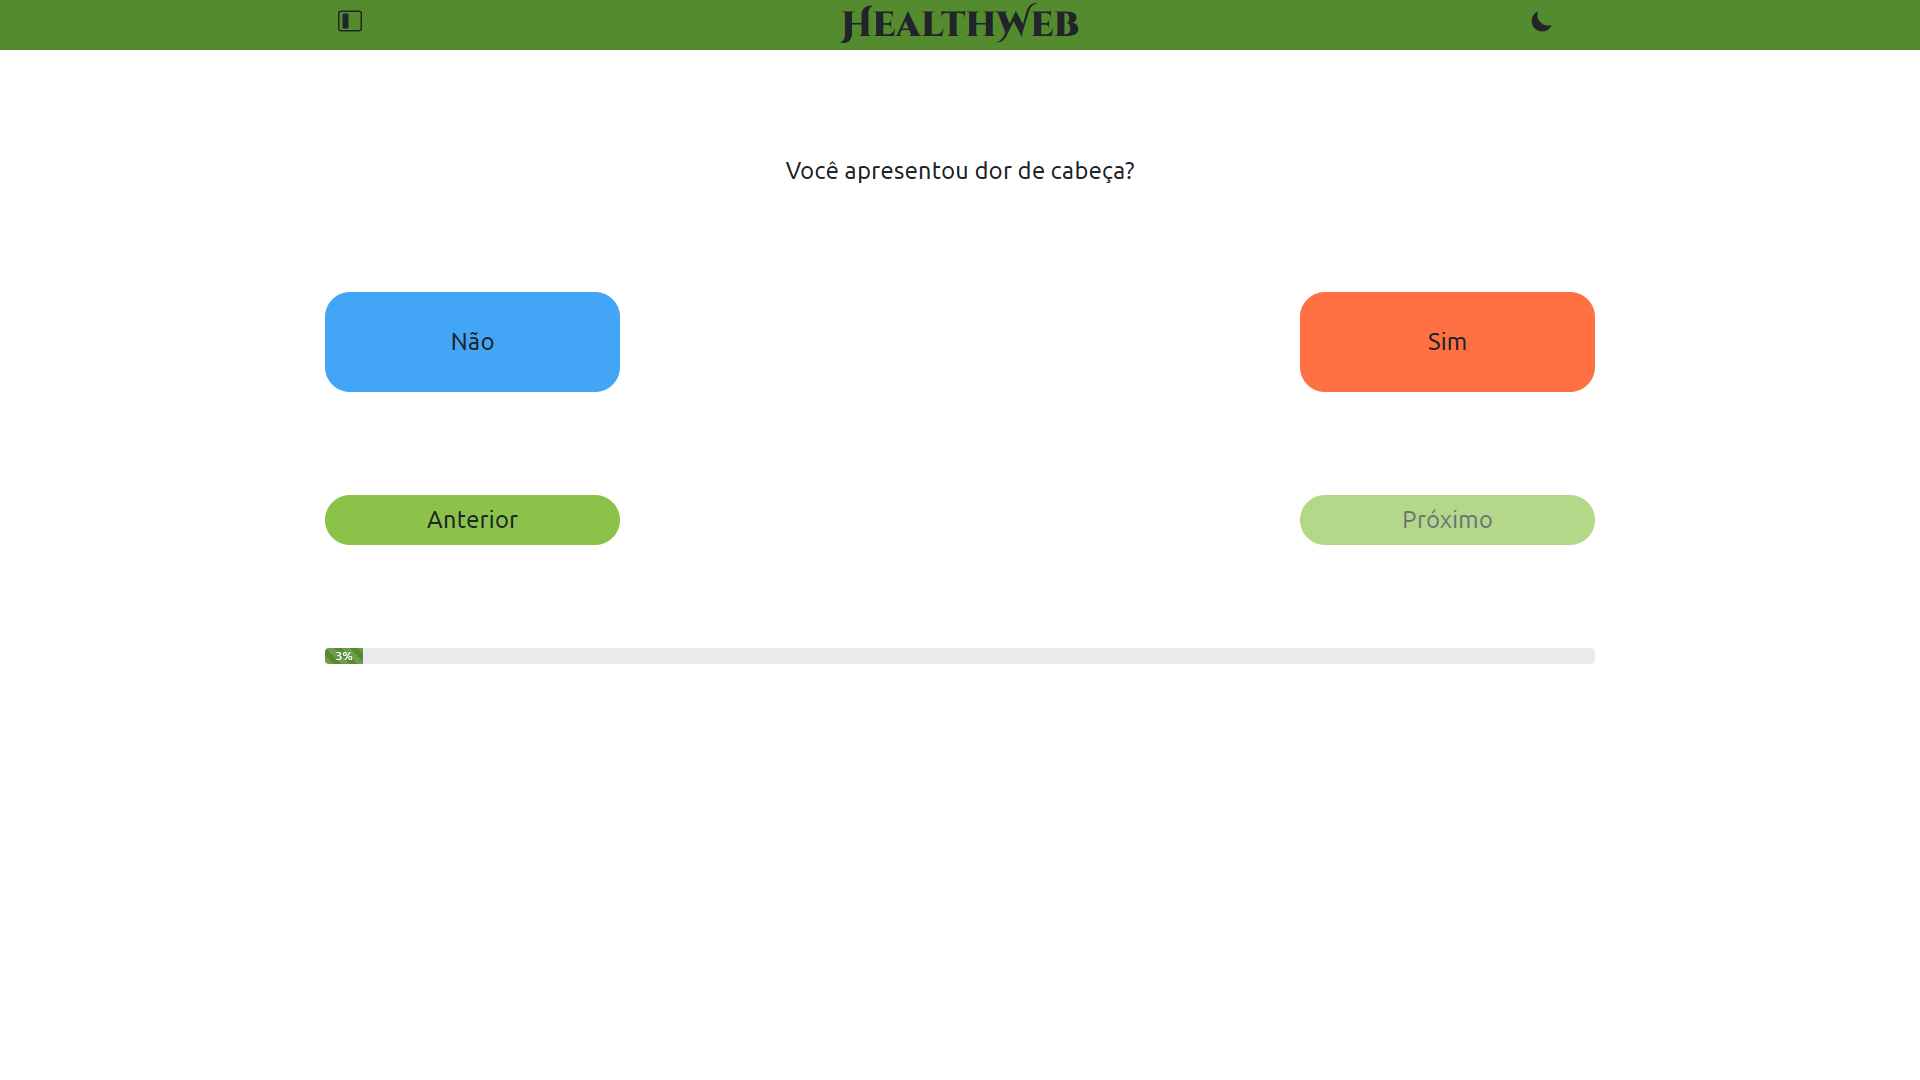
\includegraphics[width=\linewidth]{figure/disease_real.png}
		\caption{Tela de início.}
		\label{fig:desktop:disease_real}
	\end{subfigure}
	\hfill
	\begin{subfigure}{0.49\linewidth}
		\centering
		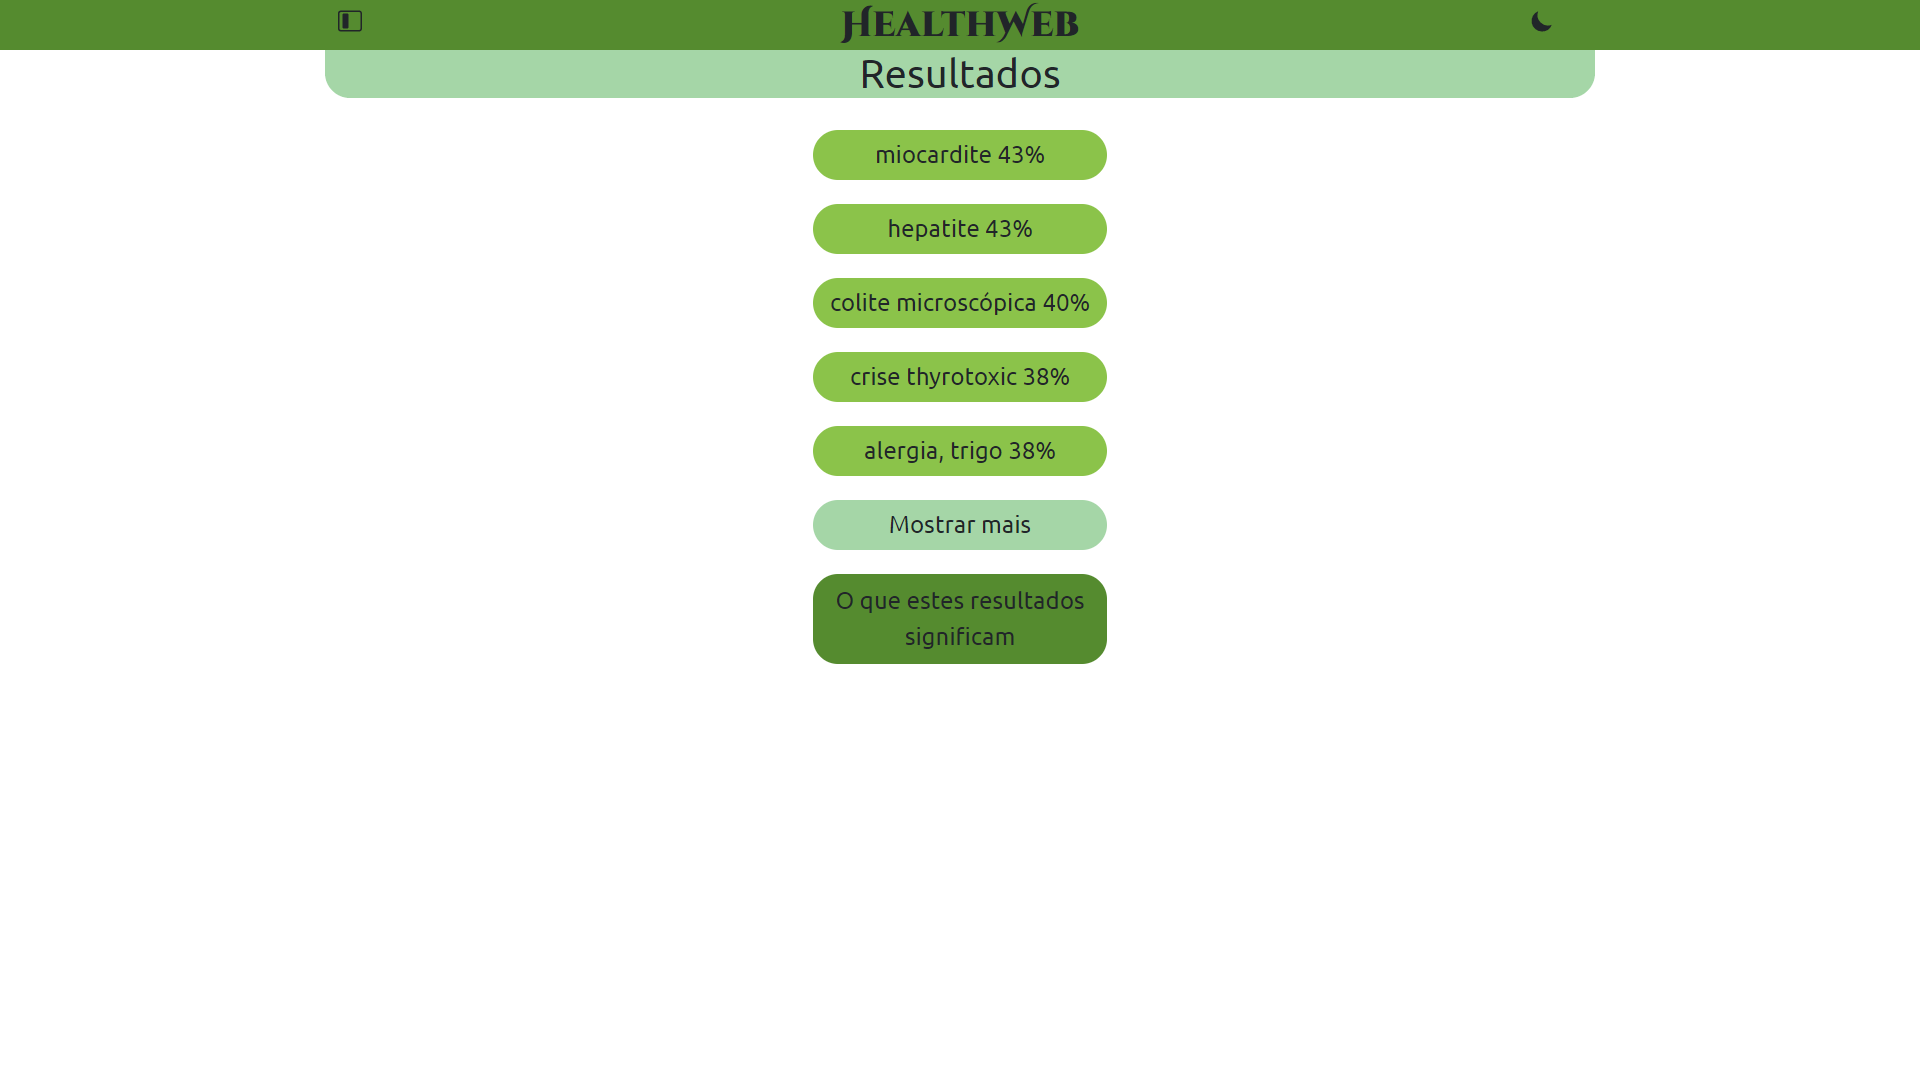
\includegraphics[width=\linewidth]{figure/results_real.png}
		\caption{Menu lateral recolhido na tela de início.}
		\label{fig:desktop:results_real}
	\end{subfigure}
	\caption{Tela de início e detalhe do menu lateral.}
	\label{fig:desktop:final}
\end{figure}




%Avaliação: A avaliação da aplicação seria feita de forma ideal recebendo respostas de um paciente e validando o diagnóstico com um médico capacitado. Embora seja possível mensurar a efetividade com casos de teste, se escolhem doenças e inserindo respostas relacionadas ao sintomas da mesma, não deixando de conferir casos excepcionais, ou  em outras palavras, casos em que o usuário possa estar com sintomas divergentes.
%Podem haver testes com usuários voluntários e até opiniões médicas.
